\begin{figure}[t]
  \hspace{0.05\textwidth}%
  \begin{subfigure}[b]{\textwidth}
    \tikzstyle{legend-point}=[circle, inner sep=2pt]
    \definecolor{Graph1}{HTML}{6c8abd}
    \definecolor{Graph2}{HTML}{73b584}
    \definecolor{Graph3}{HTML}{d07175}
    \definecolor{Graph4}{HTML}{B8DBF4}
    \definecolor{Graph5}{HTML}{ccb974}
    \definecolor{Graph6} {HTML}{64b5cd}
    \definecolor{Graph7}{HTML}{DABDE4}
    \definecolor{Graph8}{HTML}{8172b2}
    
    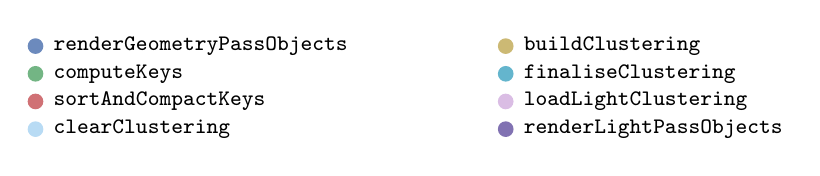
\begin{tikzpicture}
      \node (legend:1) at (0.1\textwidth,0) [legend-point, fill={Graph1}, label=right:{\footnotesize $\mathtt{renderGeometryPassObjects}$}] {};
      \node (legend:2) at (0.1\textwidth, -10pt) [legend-point, fill={Graph2}, label=right:{\footnotesize $\mathtt{computeKeys}$}] {};
      \node (legend:3) at (0.1\textwidth, -20pt) [legend-point, fill={Graph3}, label=right:{\footnotesize $\mathtt{sortAndCompactKeys}$}] {};
      \node (legend:4) at (0.1\textwidth, -30pt) [legend-point, fill={Graph4}, label=right:{\footnotesize $\mathtt{clearClustering}$}] {};
      
      \node (legend:5) at (0.5925\textwidth, -0pt) [legend-point, fill={Graph5}, label=right:{\footnotesize $\mathtt{buildClustering}$}] {};
      \node (legend:6) at (0.5925\textwidth, -10pt) [legend-point, fill={Graph6}, label=right:{\footnotesize $\mathtt{finaliseClustering}$}] {};
      \node (legend:7) at (0.5925\textwidth, -20pt) [legend-point, fill={Graph7}, label=right:{\footnotesize $\mathtt{loadLightClustering}$}] {};
      \node (legend:8) at (0.5925\textwidth, -30pt) [legend-point, fill={Graph8}, label=right:{\footnotesize $\mathtt{renderLightPassObjects}$}] {};
    \end{tikzpicture}
  \end{subfigure}\hfill\\
  \begin{adjustbox}{minipage=\textwidth, scale=0.55}
    \begin{subfigure}[b]{0.8\textwidth}
      \centering
      \def\svgwidth{\textwidth}
      \input{./img/raw/cs-frames-stacked/frames_spaceship-indoor_320.pdf_tex}
      \caption{Spaceship indoor: $70$ lichten, $320^2$ pixels.}
      \label{fig:cs-frames-stacked:indoor-70}
    \end{subfigure}
  \end{adjustbox}\hspace{-0.075\textwidth}  %
  %
  \begin{adjustbox}{minipage=\textwidth, scale=0.55}
    \begin{subfigure}[b]{0.8\textwidth}
      \centering
      \def\svgwidth{\textwidth}
      \input{./img/raw/cs-frames-stacked/frames_spaceship-indoor_2560.pdf_tex}
      \caption{Spaceship indoor: $1260$ lichten, $2560^2$ pixels.}
      \label{fig:cs-frames-stacked:indoor-2560}
    \end{subfigure}
  \end{adjustbox} \\
  %
  \begin{adjustbox}{minipage=\textwidth, scale=0.55}
    \begin{subfigure}[b]{0.8\textwidth}
      \centering
      \def\svgwidth{\textwidth}
      \input{./img/raw/cs-frames-stacked/frames_spaceship-indoor_320.pdf_tex}
      \caption{Pipers Alley: $58$ lichten, $320^2$ pixels.}
      \label{fig:cs-frames-stacked:alley-320}
    \end{subfigure}
  \end{adjustbox}\hspace{-0.075\textwidth}  %
  %
  \begin{adjustbox}{minipage=\textwidth, scale=0.55}
    \begin{subfigure}[b]{0.8\textwidth}
      \centering
      \def\svgwidth{\textwidth}
      \input{./img/raw/cs-frames-stacked/frames_pipers-alley_2560.pdf_tex}
      \caption{Pipers Alley: $1044$ lichten, $2560^2$ pixels.}
      \label{fig:cs-frames-stacked:alley-2560}
    \end{subfigure}
  \end{adjustbox} \\
  %
  \begin{adjustbox}{minipage=\textwidth, scale=0.55}
    \begin{subfigure}[b]{0.8\textwidth}
      \centering
      \def\svgwidth{\textwidth}
      \input{./img/raw/cs-frames-stacked/frames_ziggurat-city_320.pdf_tex}
      \caption{Ziggoerat Stad: $65$ lichten, $320^2$ pixels.}
      \label{fig:cs-frames-stacked:city-320}
    \end{subfigure}
  \end{adjustbox}\hspace{-0.075\textwidth}  %
  %
  \begin{adjustbox}{minipage=\textwidth, scale=0.55}
    \begin{subfigure}[b]{0.8\textwidth}
      \centering
      \def\svgwidth{\textwidth}
      \input{./img/raw/cs-frames-stacked/frames_ziggurat-city_2560.pdf_tex}
      \caption{Ziggoerat stad: $1170$ lichten, $2560$ pixels.}
      \label{fig:cs-frames-stacked:city-2560}
    \end{subfigure}
  \end{adjustbox}
  \caption{Overzicht van de uitvoeringstijd voor Deferred Clustered Shading per frame voor de
           drie testscenes bij verschillende resolutie en groottes van aantal
           lichten.}
  \label{fig:cs-frames-stacked}
\end{figure}

